\documentclass[11pt,a4paper]{article}
\usepackage[margin=24mm]{geometry}
\usepackage[T1]{fontenc}
\usepackage{graphicx,booktabs,amsmath,float,longtable,array}
\usepackage[colorlinks=true,linkcolor=blue,citecolor=blue,urlcolor=blue]{hyperref}
% Derived from saved CSV/JSON evidence.
\newcommand{\AParams}{164,962}
\newcommand{\AAccuracy}{94.30}
\newcommand{\AEpochTime}{3.246}
\newcommand{\ALatency}{1.358}
\newcommand{\ASizeKiB}{654.46}
\newcommand{\ASizeMiB}{0.639}
\newcommand{\ABestEpoch}{18}
\newcommand{\ABestVal}{94.00}
\newcommand{\AFinalTrain}{96.13}
\newcommand{\AFinalVal}{91.80}
\newcommand{\AFirstTrainLoss}{0.845}
\newcommand{\ALastTrainLoss}{0.112}
\newcommand{\ALastValLoss}{0.252}
\newcommand{\AWorstDrop}{13.36}
\newcommand{\BParams}{22,426}
\newcommand{\BAccuracy}{94.15}
\newcommand{\BEpochTime}{3.646}
\newcommand{\BLatency}{1.723}
\newcommand{\BSizeKiB}{104.09}
\newcommand{\BSizeMiB}{0.102}
\newcommand{\BBestEpoch}{23}
\newcommand{\BBestVal}{93.09}
\newcommand{\BFinalTrain}{95.52}
\newcommand{\BFinalVal}{92.00}
\newcommand{\BFirstTrainLoss}{0.975}
\newcommand{\BLastTrainLoss}{0.129}
\newcommand{\BLastValLoss}{0.250}
\newcommand{\BWorstDrop}{2.81}
\newcommand{\MobileParams}{2,236,682}
\newcommand{\MobileAccuracy}{97.31}
\newcommand{\MobileEpochTime}{7.002}
\newcommand{\MobileLatency}{8.452}
\newcommand{\MobileSizeKiB}{8964.57}
\newcommand{\MobileSizeMiB}{8.754}
\newcommand{\MobileBestEpoch}{10}
\newcommand{\MobileBestVal}{97.51}
\newcommand{\MobileFinalTrain}{99.17}
\newcommand{\MobileFinalVal}{97.51}
\newcommand{\MobileFirstTrainLoss}{0.594}
\newcommand{\MobileLastTrainLoss}{0.027}
\newcommand{\MobileLastValLoss}{0.080}
\newcommand{\MobileHeadVal}{90.84}
\newcommand{\MobileFineGain}{6.67}
\newcommand{\EfficientParams}{4,020,358}
\newcommand{\EfficientAccuracy}{96.81}
\newcommand{\EfficientEpochTime}{9.793}
\newcommand{\EfficientLatency}{12.454}
\newcommand{\EfficientSizeKiB}{15978.59}
\newcommand{\EfficientSizeMiB}{15.604}
\newcommand{\EfficientBestEpoch}{8}
\newcommand{\EfficientBestVal}{96.86}
\newcommand{\EfficientFinalTrain}{98.28}
\newcommand{\EfficientFinalVal}{96.67}
\newcommand{\EfficientFirstTrainLoss}{0.773}
\newcommand{\EfficientLastTrainLoss}{0.050}
\newcommand{\EfficientLastValLoss}{0.107}
\newcommand{\EfficientHeadVal}{89.78}
\newcommand{\EfficientFineGain}{7.09}
\newcommand{\BMargin}{77,574}
\newcommand{\ParamReduction}{86.41}
\newcommand{\StorageReduction}{84.09}
\newcommand{\MacReduction}{80.02}
\newcommand{\CustomAccuracyGap}{0.15}
\newcommand{\CustomCorrectGap}{6}
\newcommand{\BTrainingIncrease}{12.31}
\newcommand{\BCpuIncrease}{26.88}
\newcommand{\MobileAccuracyGap}{3.16}
\newcommand{\MobileParamSaving}{99.00}
\newcommand{\MobileStorageSaving}{98.84}
\newcommand{\MobileMacSaving}{74.70}
\newcommand{\EfficientAccuracyGap}{2.67}
\newcommand{\EfficientParamSaving}{99.44}
\newcommand{\EfficientStorageSaving}{99.35}
\newcommand{\EfficientMacSaving}{80.65}
\newcommand{\TransferAccuracyGap}{0.49}
\newcommand{\MomentumGain}{8.94}
\newcommand{\AdamMomentumGap}{0.89}
\newcommand{\SgdPilotBest}{81.63}
\newcommand{\SgdPilotFinalLoss}{0.573}
\newcommand{\MomentumPilotBest}{90.57}
\newcommand{\MomentumPilotFinalLoss}{0.277}
\newcommand{\AdamPilotBest}{91.46}
\newcommand{\AdamPilotFinalLoss}{0.246}
\newcommand{\AConvParams}{163,080}
\newcommand{\ABnParams}{592}
\newcommand{\AHeadParams}{1,290}
\newcommand{\BConvParams}{20,208}
\newcommand{\BBnParams}{928}
\newcommand{\BHeadParams}{1,290}
\newcommand{\APermanentPrecision}{82.46}
\newcommand{\BHighwayRecall}{86.67}

\setlength{\parindent}{0pt}
\setlength{\parskip}{5pt}
\setlength{\emergencystretch}{2em}
\begin{document}
\hypersetup{pageanchor=false}
\begin{titlepage}
\AddToHookNext{shipout/foreground}{%
  \put(\dimexpr\paperwidth-24mm\relax,-8mm){%
    \makebox[0pt][r]{\raisebox{-\height}{%
      \begingroup\setlength{\fboxsep}{5pt}%
      \fbox{\begin{minipage}{64mm}
        \raggedleft\footnotesize
        \textbf{Project Repository}\\[2pt]
        \href{https://github.com/aacaas5/EN3150_A03.git}{github.com/aacaas5/EN3150\_A03}
      \end{minipage}}\endgroup
    }}%
  }%
}
\centering
{\large University of Moratuwa\par}
\vspace{2cm}
{\Large EN3150 Assignment 03\par}
\vspace{0.8cm}
{\huge\bfseries Resource-Constrained CNN\\[0.3cm]for Edge Image Classification\par}
\vspace{1.8cm}
{\large Module: EN3150\par}
{\large Group name: Feature Four\par}
\vspace{1cm}
\begin{tabular}{ll}\toprule
Group member & Index number\\\midrule
{ARUNIYA R.} & {230059T}\\
{MUHAMATH M.A.A.A.} & {230416L}\\
{PIRIYATHARSAN M.} & {230491J}\\
{SNEKAN S.} & {230620G}\\\bottomrule
\end{tabular}
\vfill
{\large Experimental study and reproducible implementation\par}
\end{titlepage}
\hypersetup{pageanchor=true}
\begin{abstract}
Four CNNs are evaluated on a deterministic stratified 70/15/15 split of 27,000
EuroSAT RGB images, using $64\times64$ inputs. Model A uses standard convolutions;
Model B replaces later convolutions with depthwise-separable blocks. A controlled
optimizer comparison selects Adam, and both custom models are trained for 25
epochs. Model B has \BParams{} trainable parameters and achieves
\BAccuracy\% test accuracy, compared with \AAccuracy\% for Model A.
ImageNet-pretrained MobileNetV2 and EfficientNet-B0 achieve \MobileAccuracy\%
and \EfficientAccuracy\%, respectively, after two-stage fine-tuning.
Model B reduces parameters by \ParamReduction\% relative to Model A, but does
not improve its measured host latency. The results show a storage--accuracy
trade-off and demonstrate why arithmetic counts alone cannot predict runtime.
\end{abstract}
\tableofcontents
\clearpage
\section{Introduction}
CNNs learn local spatial features using shared convolution kernels \cite{lecun1998}.
Edge image classification requires a balance between recognition quality,
stored weights, computation and measured execution time. This study compares
a standard CNN (Model A), a custom depthwise-separable CNN (Model B), and two
ImageNet-pretrained lightweight networks on one fixed EuroSAT split. The central
constraint is fewer than 100,000 trainable parameters for Model B.
Experiments use PyTorch \cite{pytorch2019}; no test samples influence optimizer
selection, training, or checkpoint selection. The goal is to determine which
resources the custom sub-100k model saves and what accuracy cost is observed,
then compare that trade-off with pretrained MobileNetV2 and EfficientNet-B0.

\section{Dataset and Data Preparation}
\subsection{EuroSAT Dataset}
EuroSAT comprises Sentinel-2 satellite scenes for land-use and land-cover
classification \cite{helber2019}. We use the RGB version exposed by
\texttt{torchvision.datasets.EuroSAT}, preserving its original class labels.
\subsection{Dataset Classes}
Table~\ref{tab:dataset} lists all ten original classes and their sample counts.
Class sizes differ, so macro precision and recall complement overall accuracy
by giving equal weight to each class. EuroSAT is the only dataset used for
task-specific training and testing; CIFAR-10 is not used.
% Generated from saved experiment evidence; do not edit values.
\begin{table}[H]\centering\small
\caption{EuroSAT class counts and the shared stratified allocation.}\label{tab:dataset}
\begin{tabular}{lrrrr}
\toprule
Class & Total & Train & Validation & Test \\ \midrule
AnnualCrop & 3000 & 2100 & 450 & 450 \\
Forest & 3000 & 2100 & 450 & 450 \\
HerbaceousVegetation & 3000 & 2100 & 450 & 450 \\
Highway & 2500 & 1750 & 375 & 375 \\
Industrial & 2500 & 1750 & 375 & 375 \\
Pasture & 2000 & 1400 & 300 & 300 \\
PermanentCrop & 2500 & 1750 & 375 & 375 \\
Residential & 3000 & 2100 & 450 & 450 \\
River & 2500 & 1750 & 375 & 375 \\
SeaLake & 3000 & 2100 & 450 & 450 \\
Total & 27000 & 18900 & 4050 & 4050 \\
\bottomrule
\end{tabular}
\end{table}


\subsection{64x64 Input}
All networks receive original $64\times64$ RGB images. The pretrained networks
support this size through adaptive pooling; their usual larger ImageNet input
recipe is not used. No images are upscaled above the assignment resolution cap.
\subsection{70/15/15 Split}
One stratified split is constructed with seed 3150: training receives 70\%,
and the held-out 30\% is divided equally into validation and test sets. This
gives 18,900 training, 4,050 validation and 4,050 test images, as shown in
Table~\ref{tab:dataset}.
Actual sample indices are saved as \texttt{train\_indices.json},
\texttt{val\_indices.json} and \texttt{test\_indices.json}, alongside a
path/label manifest in \texttt{data/splits/}.
Hash checks bind every run to exactly the same split and sample order.
An exhaustive content audit found no pixel-identical images across sets.
This is an image-level split; geographic independence is not established.
\subsection{Preprocessing and Augmentation}
Images are decoded into a reusable unsigned-byte cache, converted to floating
point and divided by 255. Fixed ImageNet normalization uses means
$(0.485,0.456,0.406)$ and standard deviations $(0.229,0.224,0.225)$.
Independent horizontal flips with probability 0.5 apply only during training.
Validation and test processing is deterministic. Custom and pretrained models
use the same pipeline here; neither normalization nor augmentation changes
sample membership or estimates statistics from held-out data.

\section{Custom CNN Architectures}
\subsection{Model A}
Four standard $3\times3$ convolutions use channel widths 24, 48, 96 and 128.
Each is followed by batch normalization, ReLU and $2\times2$ max-pooling.
Padding preserves convolutional spatial size. Global average pooling and a
small linear head avoid a large flattened dense layer. Batch normalization
provides learned channel scaling and stabilizes intermediate feature scales.
Table~\ref{tab:model_a_layers} gives every layer's input/output shape, kernel,
stride, padding, activation and parameter count. The total is \AParams{};
all parameters are trainable. The linear head outputs ten unnormalized logits
for cross-entropy loss.

\subsection{Model B}
The stem, channel widths, pooling schedule and head match Model A. Each later
standard convolution is replaced by a depthwise $3\times3$ convolution followed
by a pointwise $1\times1$ convolution. Depthwise groups equal input channels.
Each component has batch normalization and ReLU. These extra operations mean
this is not a strict single-operator ablation. Table~\ref{tab:model_b_layers}
identifies depthwise and pointwise operations separately. Channel counts are
the second dimension of each NCHW shape, and activations are shown as separate
rows. Model B is built from scratch using a reusable
\texttt{DepthwiseSeparableConv} block.

The executed count is \BParams{} trainable parameters, leaving
\BMargin{} below the 100,000 limit. The constructor and verification script
check this programmatically:
\begin{verbatim}
count = sum(p.numel() for p in model.parameters()
            if p.requires_grad)
assert count < 100000
\end{verbatim}
The sum of the layer counts in Table~\ref{tab:model_b_layers} independently
agrees with this result.

\subsection{Depthwise Separable Convolution}
Depthwise filtering processes channels independently; pointwise convolution
learns cross-channel combinations \cite{howard2017}. For output spatial size
$H_o\times W_o$, multiplying the weight expressions below by $H_oW_o$ gives
the corresponding convolution MAC counts for one image.
Here a MAC is one multiply--accumulate operation. The factorization reduces
the number of weights because a separate spatial kernel is no longer learned
for every input--output channel pair. It also restricts the possible filters,
so equal accuracy is not guaranteed.
\subsection{Parameter Calculation}
With convolution biases disabled,
\begin{align}
P_{\mathrm{standard}} &= K_hK_wC_{\mathrm{in}}C_{\mathrm{out}},\label{eq:standard}\\
P_{\mathrm{DSC}} &= K_hK_wC_{\mathrm{in}} + C_{\mathrm{in}}C_{\mathrm{out}}.\label{eq:dsc}
\end{align}
In Equations~\eqref{eq:standard} and~\eqref{eq:dsc}, $K_h,K_w$ are kernel
dimensions and $C_{\mathrm{in}},C_{\mathrm{out}}$ are channel counts. Dividing
the two expressions gives
\begin{equation}
\frac{P_{\mathrm{DSC}}}{P_{\mathrm{standard}}}
=\frac{1}{C_{\mathrm{out}}}+\frac{1}{K_hK_w},
\qquad
\text{reduction}=100\left(1-\frac{P_{\mathrm{DSC}}}{P_{\mathrm{standard}}}\right)\%.
\label{eq:reduction}
\end{equation}
Table~\ref{tab:savings} applies Equation~\eqref{eq:reduction} to the three
replaced convolutions. Batch normalization adds two
trainable scalars per output channel; running statistics are non-trainable
buffers. The classification head includes bias. Thus whole-network counts
include more than the convolution weights in this table.
% Generated from saved experiment evidence; do not edit values.
\begin{table}[H]\centering\small
\caption{Convolution weight counts excluding bias and normalization; reduction compares depthwise plus pointwise with standard convolution.}\label{tab:savings}
\begin{tabular}{lrrrr}
\toprule
Channels & Standard & Depthwise & Pointwise & Reduction (\%) \\ \midrule
24 to 48 & 10368 & 216 & 1152 & 86.81 \\
48 to 96 & 41472 & 432 & 4608 & 87.85 \\
96 to 128 & 110592 & 864 & 12288 & 88.11 \\
\bottomrule
\end{tabular}
\end{table}

Summing the executed architecture tables gives \AConvParams{} convolution
weights, \ABnParams{} normalization parameters and \AHeadParams{} head
parameters for Model A, totalling \AParams{}. The corresponding Model B
counts are \BConvParams{}, \BBnParams{} and \BHeadParams{}, totalling
\BParams{}. Whole-network savings differ from an individual convolution's
savings because the stem and head are retained and Model B adds normalization.

\subsection{Hardware-Aware Activation Selection}
ReLU computes $\max(0,x)$ using a simple comparison and avoids exponentials.
It is widely supported by inference kernels and is compatible with common
integer inference workflows. No quantization or activation-specific energy
measurement is performed here, so hardware savings are not claimed empirically.
ReLU is the deliberate choice for both custom networks. The pretrained
architectures retain their original activations: MobileNetV2 uses ReLU6,
whereas EfficientNet-B0 uses SiLU and sigmoid operations. They are not modified
to match the custom networks.

\section{Optimizer Selection and Tuning}
\subsection{SGD}
Standard SGD updates parameters with the current minibatch gradient. The
baseline uses learning rate 0.01 and no momentum.
\subsection{SGD with Momentum}
Momentum accumulates a velocity from earlier gradients; this can accelerate
consistent descent directions \cite{sutskever2013}. The experiment uses
learning rate 0.01 and momentum 0.9, without Nesterov acceleration.
For minibatch gradient $g_t$, the update can be written as
\begin{equation}
v_t=\mu v_{t-1}+g_t,\qquad
\theta_{t+1}=\theta_t-\eta v_t,
\label{eq:momentum}
\end{equation}
where $\eta$ is the learning rate and $\mu$ is the momentum coefficient.
Equation~\eqref{eq:momentum} reduces to standard SGD when $\mu=0$.
Accumulating gradients can smooth inconsistent directions, although it does
not guarantee a smoother validation curve.
\subsection{Adam}
Adam adapts updates using first and second gradient moments \cite{kingma2015}.
The tested learning rate is 0.001, with default betas $(0.9,0.999)$ and
$\epsilon=10^{-8}$.
\subsection{Experimental Comparison}
Model B is used for its low compute requirement. Each recipe uses ten epochs,
batch size 128, identical initial weights, seed, data order and augmentation
strategy. No weight decay, scheduler or early stopping is used. These are
controlled recipe comparisons, not exhaustive learning-rate searches.
Table~\ref{tab:optimizers} records settings, best validation performance and
final validation accuracy; Table~\ref{tab:optimizer_dynamics} adds final losses
and timing. ``Final'' here means the last pilot epoch, not a test-set result.
The pilot test sets are not evaluated for optimizer selection.
% Generated from saved experiment evidence; do not edit values.
\begin{table}[H]\centering\small
\caption{Optimizer comparison on Model B; each run uses ten epochs. Adam moment coefficients are specified in the text.}\label{tab:optimizers}
\begin{tabular}{lrrrrr}
\toprule
Optimizer & LR & Momentum & Best val. (\%) & Epoch & Final val. (\%) \\ \midrule
Adam & 0.001 & -- & 91.46 & 10 & 91.46 \\
SGD + momentum & 0.01 & 0.9 & 90.57 & 8 & 90.52 \\
SGD & 0.01 & 0 & 81.63 & 9 & 80.05 \\
\bottomrule
\end{tabular}
\end{table}

% Generated from saved experiment evidence; do not edit values.
\begin{table}[H]\centering\small
\caption{Final-epoch optimizer losses and training accuracy; mean timing spans all ten epochs.}\label{tab:optimizer_dynamics}
\begin{tabular}{lrrrr}
\toprule
Optimizer & Train loss & Val. loss & Train acc. (\%) & Epoch (s) \\ \midrule
SGD & 0.545 & 0.573 & 81.52 & 3.164 \\
SGD + momentum & 0.250 & 0.277 & 91.35 & 2.963 \\
Adam & 0.220 & 0.246 & 92.30 & 3.078 \\
\bottomrule
\end{tabular}
\end{table}

Figure~\ref{fig:optimizer_comparison} shows that plain SGD improves gradually
but finishes with higher validation loss than the other recipes. Momentum
reaches a much higher validation accuracy within the same budget, despite
fluctuations during the middle epochs. Adam finishes with the lowest validation
loss, \AdamPilotFinalLoss{}, compared with \MomentumPilotFinalLoss{} for
momentum SGD and \SgdPilotFinalLoss{} for plain SGD.
\begin{figure}[H]\centering
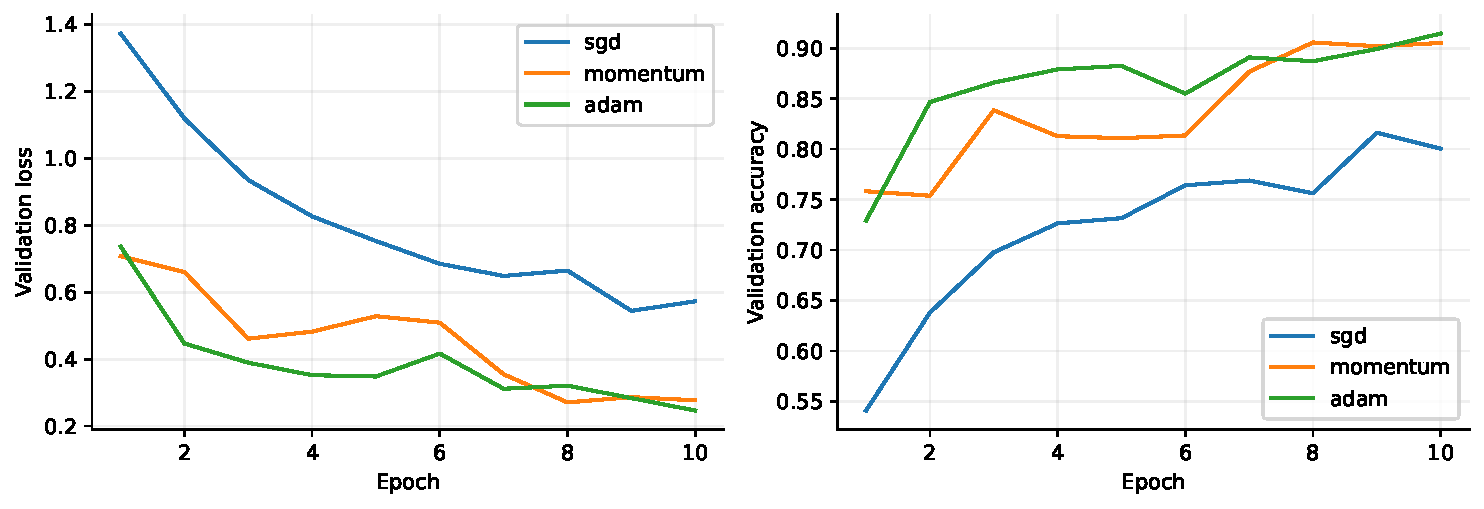
\includegraphics[width=0.96\textwidth]{figures/optimizer_comparison.pdf}
\caption{Validation loss and accuracy; unsmoothed observations.}
\label{fig:optimizer_comparison}
\end{figure}
\subsection{Selected Optimizer}
Adam is selected by highest validation accuracy, with lower validation loss
breaking ties. Its best validation accuracy is \AdamPilotBest\%, compared with
\MomentumPilotBest\% for momentum SGD and \SgdPilotBest\% for plain SGD.
Momentum therefore improves on plain SGD by \MomentumGain{} percentage points
at the same learning rate. Adam's advantage over momentum SGD is smaller,
\AdamMomentumGap{} percentage points, and also involves a different learning
rate. This experiment supports choosing Adam for the final runs; it does not
isolate optimizer type from learning-rate choice or establish universal
superiority. Losses are still improving near the end, so the fixed budget does
not establish full convergence. The initial settings were retained, and no
setting was chosen using test performance.

\section{Custom CNN Training and Evaluation}
\subsection{Training Setup}
Both custom models are initialized afresh and trained for 25 epochs using the
selected optimizer Adam at learning rate 0.001, batch size 128 and cross-entropy
loss. Thus both exceed the required minimum of 20 epochs. Computation uses
32-bit floating point (FP32) on an NVIDIA GeForce RTX 5060 Laptop GPU. Deterministic algorithms and
seed 3150 are enabled. The best validation-accuracy checkpoint, with validation
loss breaking ties, is retained. There is no early stopping. The first ten
epochs of the final Model B run exactly reproduce its Adam pilot losses and
accuracies. One reusable training loop handles the custom and pretrained
models, with configurable epochs, batch size and optimizer, CUDA support and
CPU fallback. Python 3.14.5, PyTorch 2.13.0+cu130 and torchvision 0.28.0+cu130
are recorded in each run's JSON. CSV histories contain every epoch's losses,
accuracies, stage and elapsed time. Checkpoints store the validation-selected
weights, not the final epoch by default.
\subsection{Training Curves}
Figures~\ref{fig:model_a_curves} and~\ref{fig:model_b_curves} show the complete
training histories. Both training losses decrease overall, while validation
losses fluctuate. The gap between training and validation performance near
the end suggests that continued fitting of the training set does not reliably
improve held-out performance.
\begin{figure}[H]\centering
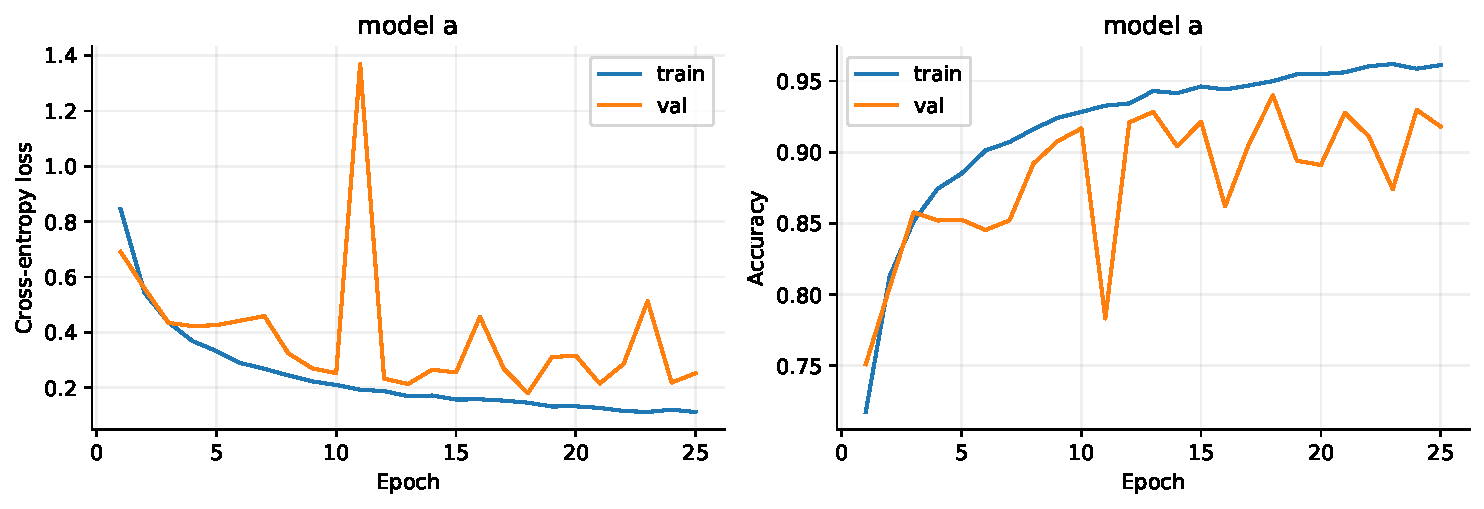
\includegraphics[width=0.96\textwidth]{figures/model_a_curves.pdf}
\caption{Model A training and validation history.}
\label{fig:model_a_curves}
\end{figure}
Model A selects epoch \ABestEpoch{} with \ABestVal\% validation accuracy.
Final training/validation accuracies are \AFinalTrain\%/\AFinalVal\%.
Its largest epoch-to-epoch validation drop is \AWorstDrop{} percentage points
at epoch 11, followed by recovery. This is a temporary instability in the
observed validation trajectory; the experiment does not identify its cause.
\begin{figure}[H]\centering
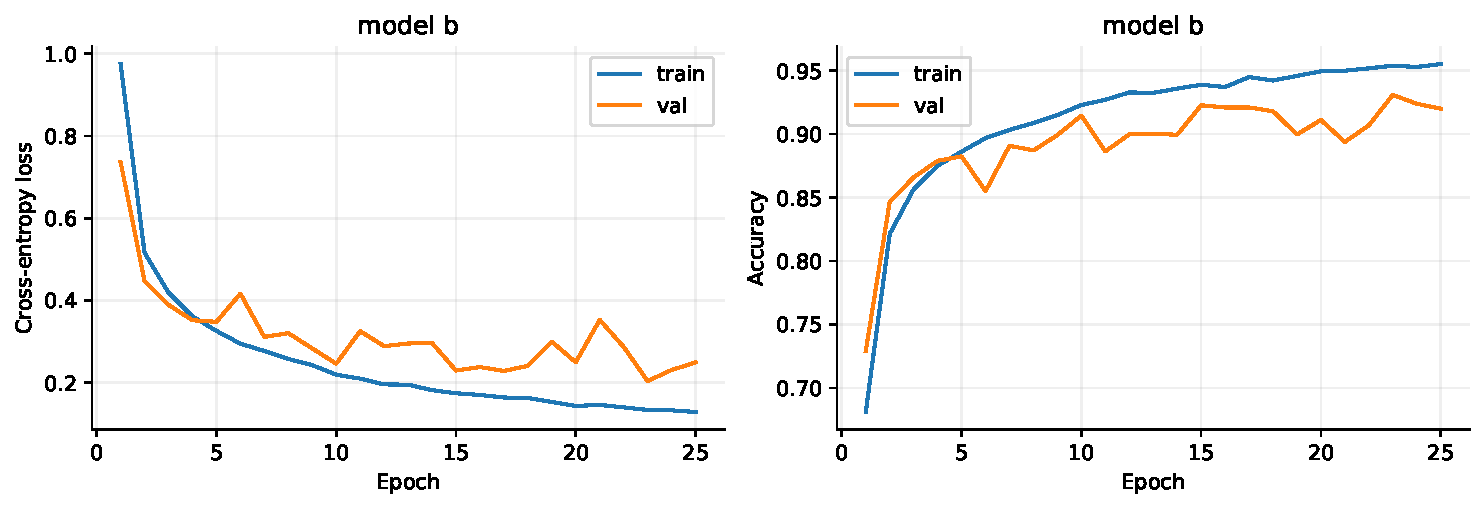
\includegraphics[width=0.96\textwidth]{figures/model_b_curves.pdf}
\caption{Model B training and validation history.}
\label{fig:model_b_curves}
\end{figure}
Model B selects epoch \BBestEpoch{} with \BBestVal\% validation accuracy.
Final training/validation accuracies are \BFinalTrain\%/\BFinalVal\%.
Its largest epoch-to-epoch validation drop is \BWorstDrop{} percentage points
at epoch 11, smaller than Model A's largest drop. However, neither run gives
a monotonic validation improvement, which supports retaining the best
validation checkpoint rather than using the last epoch automatically.
\subsection{Test Results}
Accuracy is the fraction of correct predictions. Precision and recall are
unweighted macro averages over all ten classes; undefined class precision is
set to zero. Each selected checkpoint is evaluated on the untouched test set.
For class $c$, let $TP_c$, $FP_c$ and $FN_c$ denote true positives, false
positives and false negatives. With $C=10$ classes and $N=4050$ test images,
\begin{equation}
\begin{aligned}
\mathrm{Accuracy}&=\frac{\sum_c TP_c}{N},\\
\mathrm{MacroPrecision}&=\frac{1}{C}\sum_{c=1}^{C}\frac{TP_c}{TP_c+FP_c},\\
\mathrm{MacroRecall}&=\frac{1}{C}\sum_{c=1}^{C}\frac{TP_c}{TP_c+FN_c}.
\end{aligned}\label{eq:metrics}
\end{equation}
The scikit-learn calculations in Table~\ref{tab:custom_accuracy} follow
Equation~\eqref{eq:metrics}. Model A is slightly higher on all three aggregate
metrics, but its accuracy advantage corresponds to only \CustomCorrectGap{}
additional correct predictions on this test set. This is a small observed
difference, not evidence of a consistent advantage over repeated runs.
% Generated from saved experiment evidence; do not edit values.
\begin{table}[H]\centering\small
\caption{Held-out test metrics for custom models; P is precision and R is recall.}\label{tab:custom_accuracy}
\begin{tabular}{lrrr}
\toprule
Model & Accuracy (\%) & Macro P (\%) & Macro R (\%) \\ \midrule
Model A & 94.30 & 94.25 & 94.26 \\
Model B & 94.15 & 94.00 & 93.88 \\
\bottomrule
\end{tabular}
\end{table}

\subsection{Confusion Matrices}
Figures~\ref{fig:model_a_cm} and~\ref{fig:model_b_cm} show raw counts, not row
percentages. Model A confuses HerbaceousVegetation with PermanentCrop more
often, while Model B's largest directed error is Highway predicted as
Industrial. Similar overall accuracy therefore does not imply identical
class-level behaviour; Section~\ref{sec:discussion} examines these errors.
\begin{figure}[H]\centering
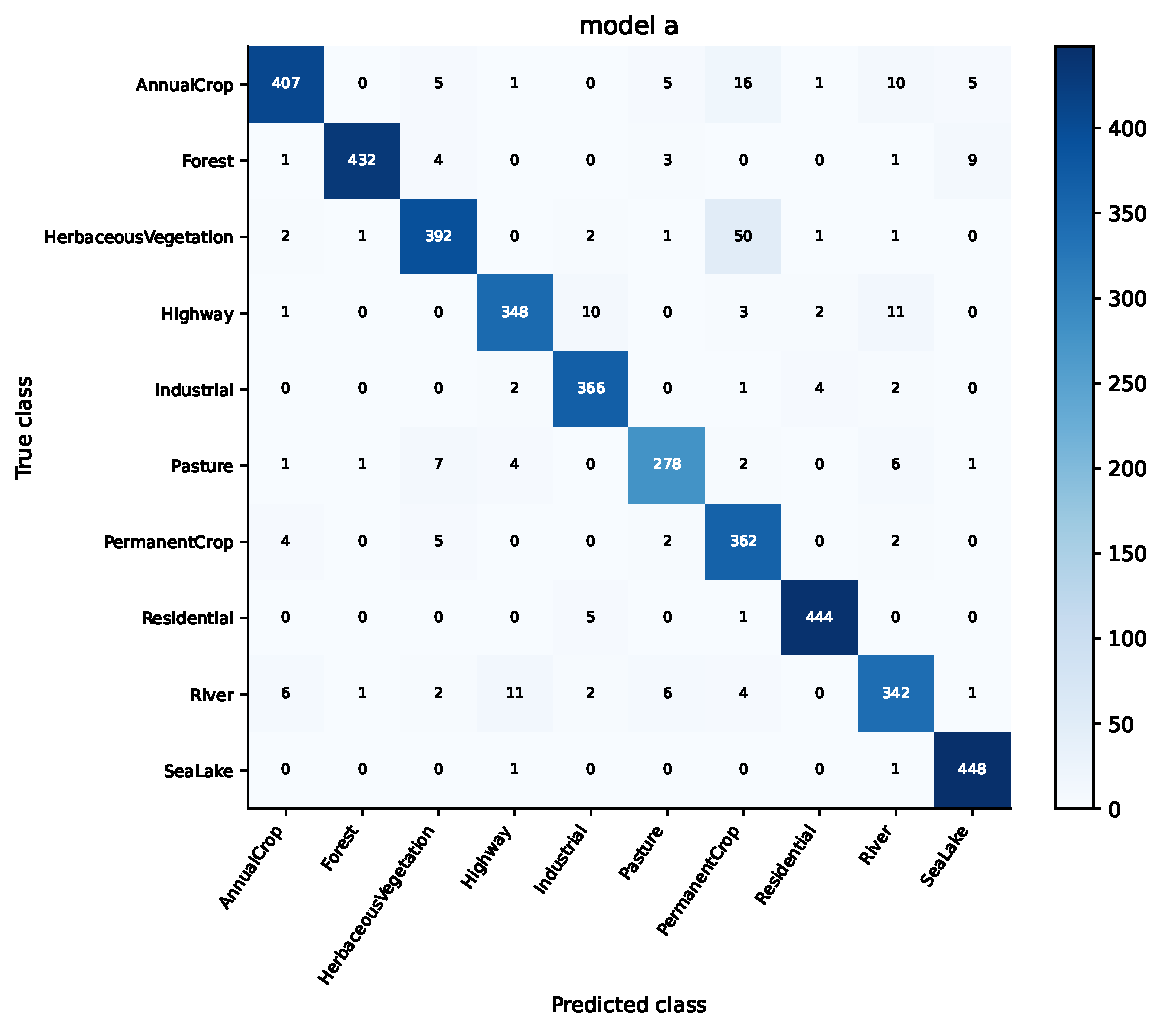
\includegraphics[width=.72\textwidth]{figures/model_a.pdf}
\caption{Model A: numeric counts, true classes on rows and predictions on columns.}
\label{fig:model_a_cm}
\end{figure}
\begin{figure}[H]\centering
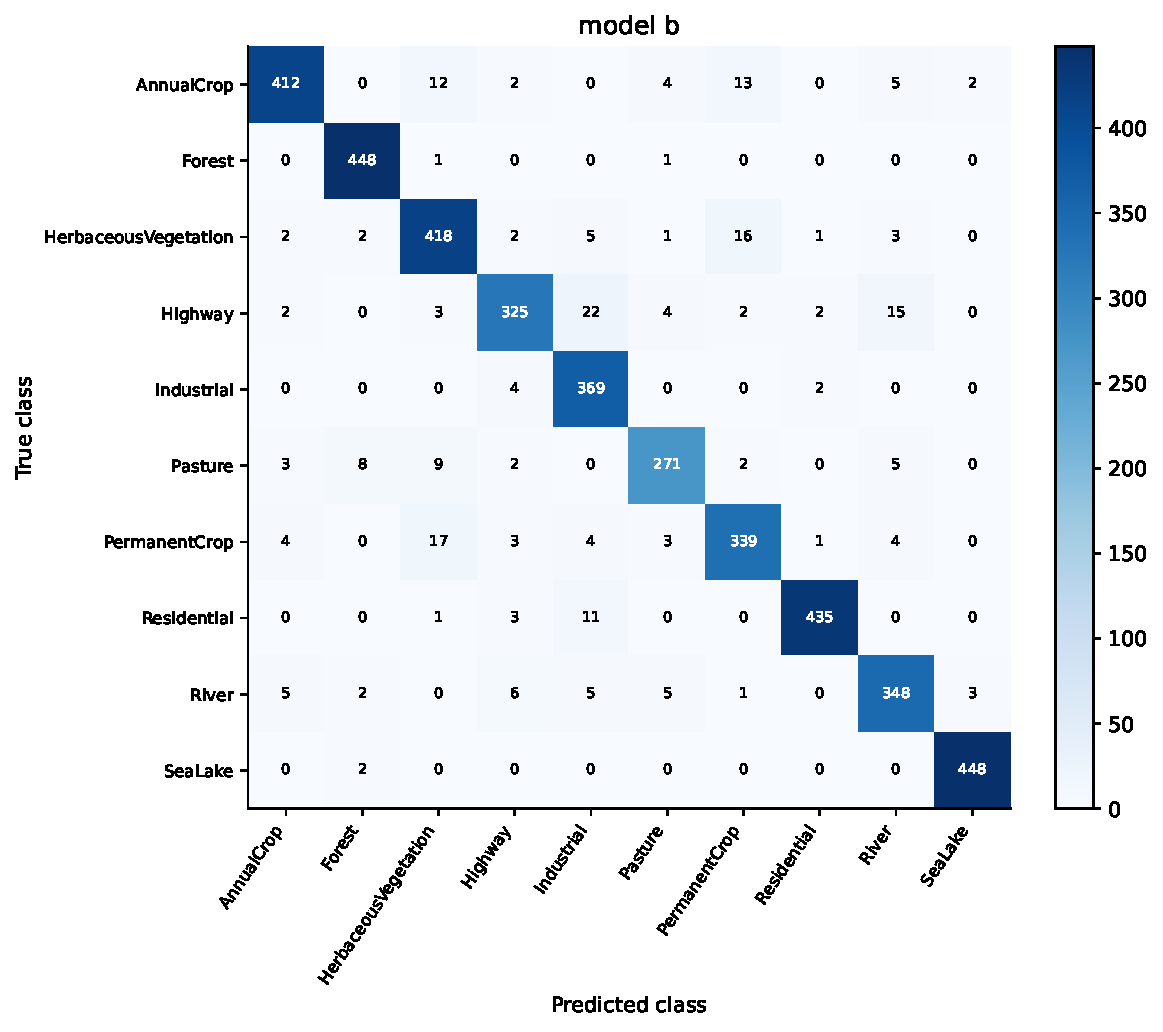
\includegraphics[width=.72\textwidth]{figures/model_b.pdf}
\caption{Model B: numeric counts, true classes on rows and predictions on columns.}
\label{fig:model_b_cm}
\end{figure}
\subsection{Model A vs Model B Resource Comparison}
Table~\ref{tab:custom_resources} compares measured checkpoint sizes and mean
epoch times with parameter and MAC counts. Timing includes training,
validation and batch preprocessing, with CUDA synchronization at the timing
boundaries; it excludes checkpoint and CSV writes. It is therefore a mean
complete-epoch time, not a training-only kernel benchmark.
% Generated from saved experiment evidence; do not edit values.
\begin{table}[H]\centering\small
\caption{Custom-model resources. All parameters are trainable; epoch time includes validation.}\label{tab:custom_resources}
\begin{tabular}{lrrrr}
\toprule
Model & Parameters & Size (KiB) & Epoch (s) & MACs (M) \\ \midrule
Model A & 164,962 & 654.46 & 3.246 & 30.967 \\
Model B & 22,426 & 104.09 & 3.646 & 6.188 \\
\bottomrule
\end{tabular}
\end{table}

Model B reduces whole-network parameters by \ParamReduction\%, serialized
size by \StorageReduction\%, and counted MACs by \MacReduction\%.
Its test accuracy is \CustomAccuracyGap{} percentage points lower. The mean
epoch time nevertheless rises from \AEpochTime{} s to \BEpochTime{} s.
Depthwise kernel efficiency, additional normalization/activation operations
and memory or launch overhead can prevent arithmetic savings from producing
speedups. These are possible explanations; the timing experiment does not
separate their contributions.

\section{Lightweight State-of-the-Art Models}
\subsection{MobileNetV2}
MobileNetV2 uses inverted residual blocks and linear bottlenecks
\cite{sandler2018}. We load torchvision's explicit ImageNet
\texttt{IMAGENET1K\_V2} weights and replace its classifier with a ten-class head.
Its depthwise layers reduce spatial filtering cost, while pointwise expansion
and projection layers mix channels. It is still much larger than Model B:
``lightweight'' does not imply compliance with the custom parameter limit.
\subsection{EfficientNet-B0}
EfficientNet balances network depth, width and resolution \cite{tan2019}.
We use torchvision's B0 \texttt{IMAGENET1K\_V1} weights and replace its final
classifier. No fallback to random initialization is permitted.
It retains inverted bottlenecks, squeeze-and-excitation channel weighting
and its original nonlinearities. The pretrained comparison includes prior
ImageNet learning as well as architectural differences.
\subsection{Transfer Learning Strategy}
Stage one trains the head for two epochs using Adam at 0.001; feature weights
and feature batch-normalization running statistics remain frozen. Stage two
unfreezes the entire network and uses a new Adam optimizer at 0.0001 for eight
epochs. Validation selects the checkpoint across both stages. Both models use
exactly the saved custom-model split and the same 64x64 preprocessing.
Table~\ref{tab:transfer_stages} distinguishes trainable counts and timing in
the frozen-head and full-network stages. Both use the shared training loop.
% Generated from saved experiment evidence; do not edit values.
\begin{table}[H]\centering\small
\caption{Transfer-learning stages, learning rates and measured mean epoch times.}\label{tab:transfer_stages}
\begin{tabular}{lrrrrr}
\toprule
Model & Stage & Epochs & LR & Trainable & Epoch (s) \\ \midrule
MobileNetV2 & head & 2 & 0.001 & 12,810 & 3.347 \\
MobileNetV2 & finetune & 8 & 0.0001 & 2,236,682 & 7.915 \\
EfficientNet-B0 & head & 2 & 0.001 & 12,810 & 4.263 \\
EfficientNet-B0 & finetune & 8 & 0.0001 & 4,020,358 & 11.175 \\
\bottomrule
\end{tabular}
\end{table}

\subsection{Results}
Table~\ref{tab:pretrained_accuracy} reports classification metrics, while
Table~\ref{tab:pretrained_resources} separates total and fine-tuning trainable
parameters, checkpoint size and epoch time. MobileNetV2 is
\TransferAccuracyGap{} percentage points more accurate than EfficientNet-B0
in this run despite having fewer parameters. A larger pretrained model does
not automatically give a better result at this input size and training budget.
% Generated from saved experiment evidence; do not edit values.
\begin{table}[H]\centering\small
\caption{Held-out test metrics for pretrained models; P is precision and R is recall.}\label{tab:pretrained_accuracy}
\begin{tabular}{lrrr}
\toprule
Model & Accuracy (\%) & Macro P (\%) & Macro R (\%) \\ \midrule
MobileNetV2 & 97.31 & 97.20 & 97.21 \\
EfficientNet-B0 & 96.81 & 96.72 & 96.71 \\
\bottomrule
\end{tabular}
\end{table}

% Generated from saved experiment evidence; do not edit values.
\begin{table}[H]\centering\small
\caption{Pretrained-model resources. Trainable counts refer to fine-tuning; timing averages both stages.}\label{tab:pretrained_resources}
\begin{tabular}{lrrrr}
\toprule
Model & Total & Trainable & Size (MiB) & Epoch (s) \\ \midrule
MobileNetV2 & 2,236,682 & 2,236,682 & 8.754 & 7.002 \\
EfficientNet-B0 & 4,020,358 & 4,020,358 & 15.604 & 9.793 \\
\bottomrule
\end{tabular}
\end{table}

Figure~\ref{fig:mobilenet_v2_curves} shows improvement from
\MobileHeadVal\% validation accuracy after head training to a best of
\MobileBestVal\% at epoch \MobileBestEpoch{}, a gain of
\MobileFineGain{} percentage points. Updating the features is therefore
useful under this schedule. Training loss increases at the first fine-tuning
epoch, coinciding with unfreezing and switching the feature extractor to
training mode. Feature batch-normalization statistics are then updated;
EfficientNet-B0 also activates stochastic depth in its feature extractor.
These changed training conditions must be considered when reading the
stage-transition losses.
\begin{figure}[H]\centering
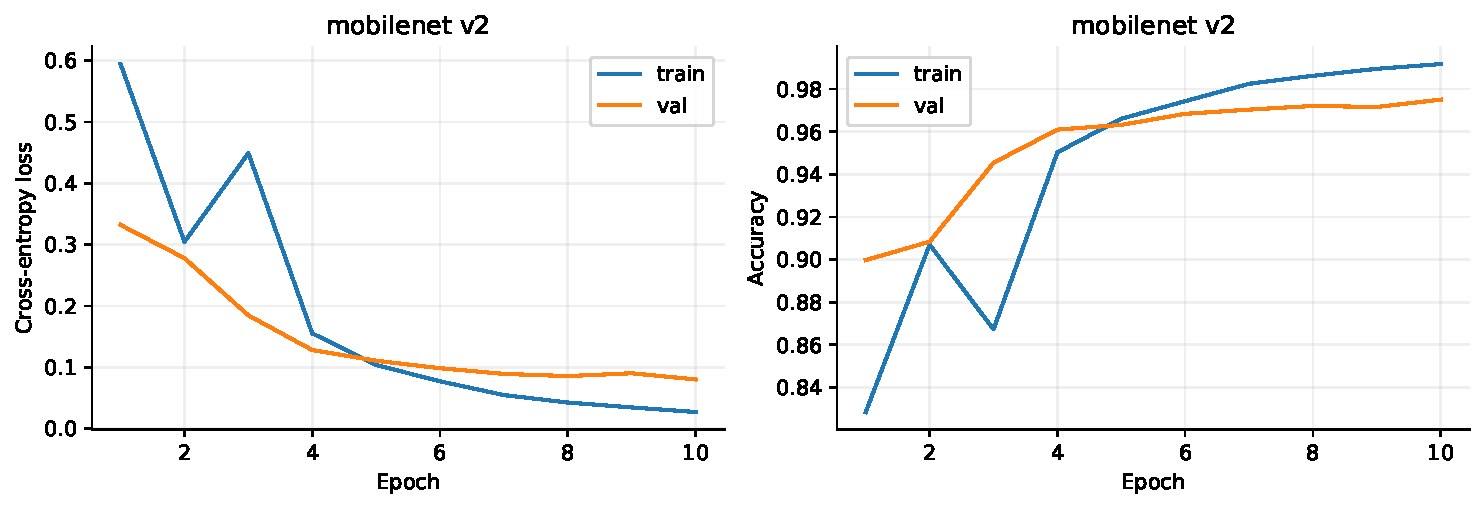
\includegraphics[width=0.96\textwidth]{figures/mobilenet_v2_curves.pdf}
\caption{MobileNetV2: frozen-head epochs 1--2 and full-network fine-tuning epochs 3--10.}
\label{fig:mobilenet_v2_curves}
\end{figure}
\begin{figure}[H]\centering
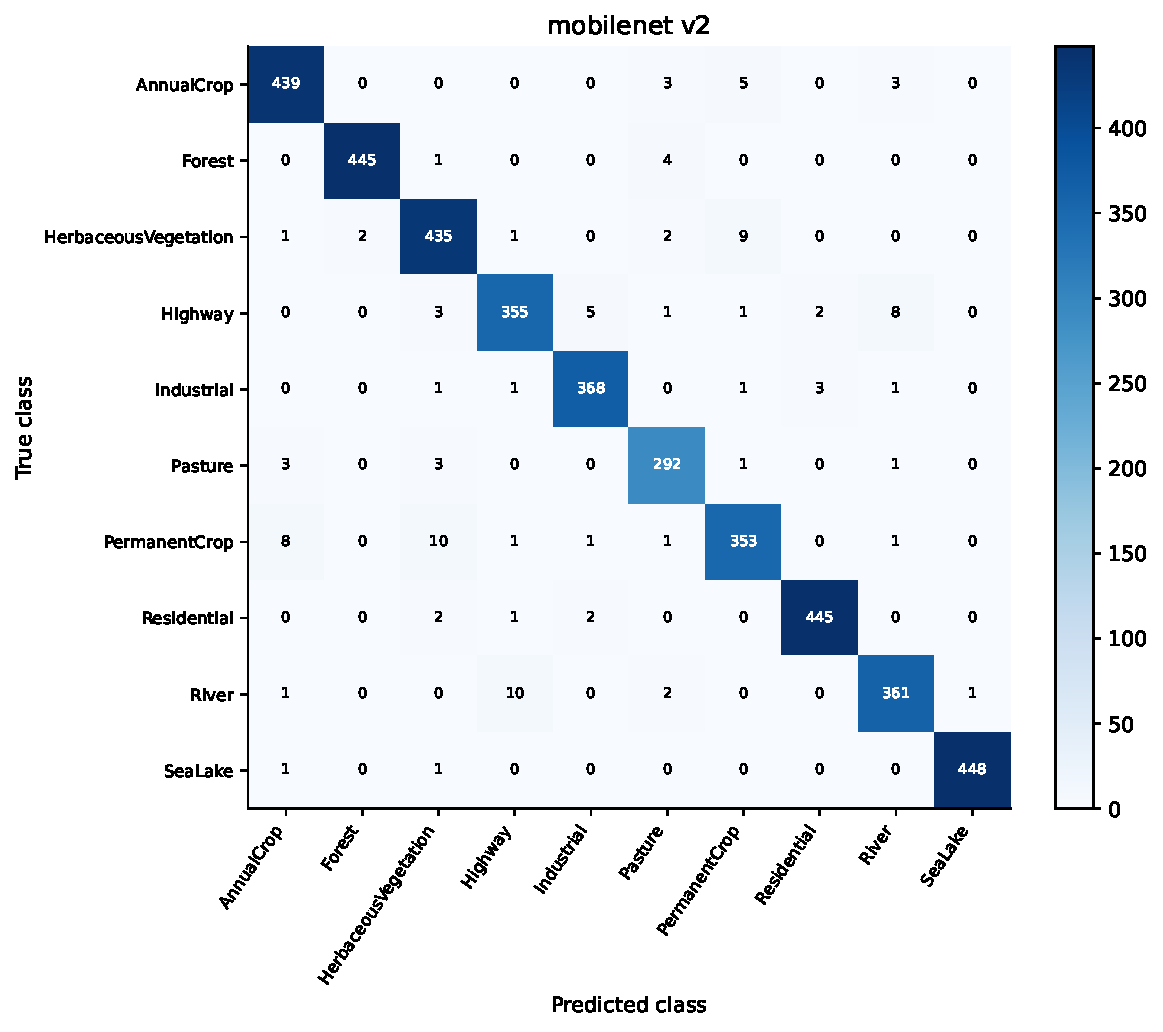
\includegraphics[width=.72\textwidth]{figures/mobilenet_v2.pdf}
\caption{MobileNetV2 test confusion matrix (counts).}
\label{fig:mobilenet_v2_cm}
\end{figure}
Figure~\ref{fig:mobilenet_v2_cm} shows MobileNetV2's remaining class errors;
Section~\ref{sec:discussion} examines the largest directed confusions.
EfficientNet-B0 improves from \EfficientHeadVal\% validation accuracy after
head training to \EfficientBestVal\% at epoch \EfficientBestEpoch{}, a gain
of \EfficientFineGain{} percentage points.
Figure~\ref{fig:efficientnet_b0_curves} shows the same stage-transition
training-loss increase, followed by improvement. Training loss continues to
fall late in the run while validation performance levels off, so its selected
checkpoint precedes the final epoch. Figure~\ref{fig:efficientnet_b0_cm}
shows its test errors, including confusion between crop classes.
\begin{figure}[H]\centering
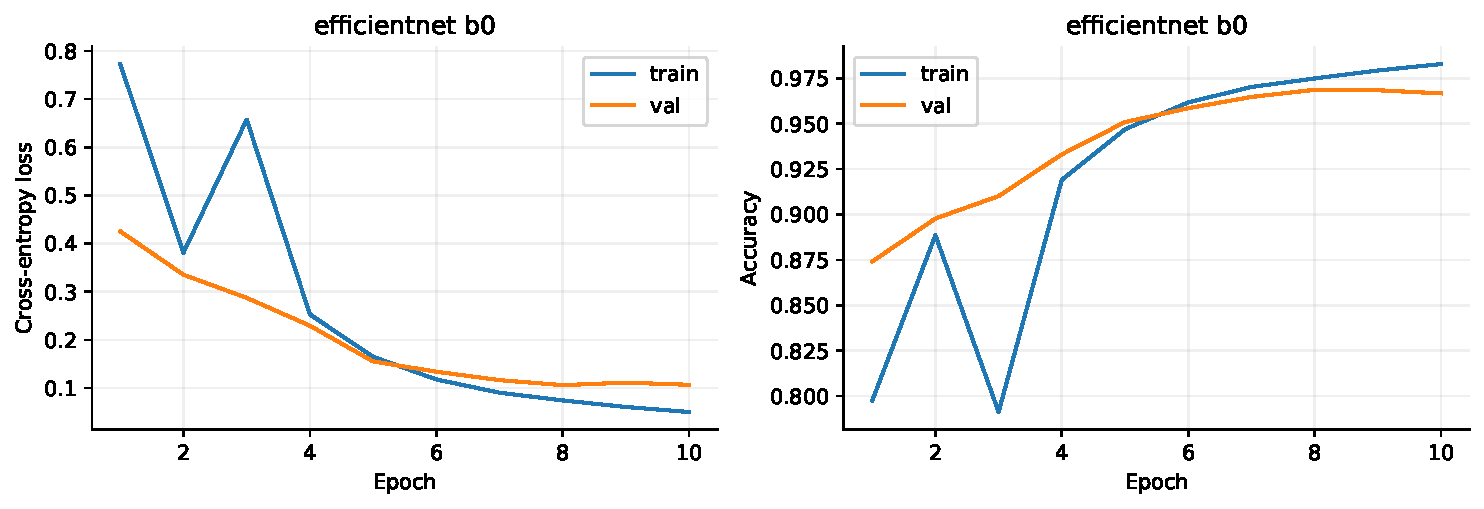
\includegraphics[width=0.96\textwidth]{figures/efficientnet_b0_curves.pdf}
\caption{EfficientNet-B0: frozen-head epochs 1--2 and full-network fine-tuning epochs 3--10.}
\label{fig:efficientnet_b0_curves}
\end{figure}
\begin{figure}[H]\centering
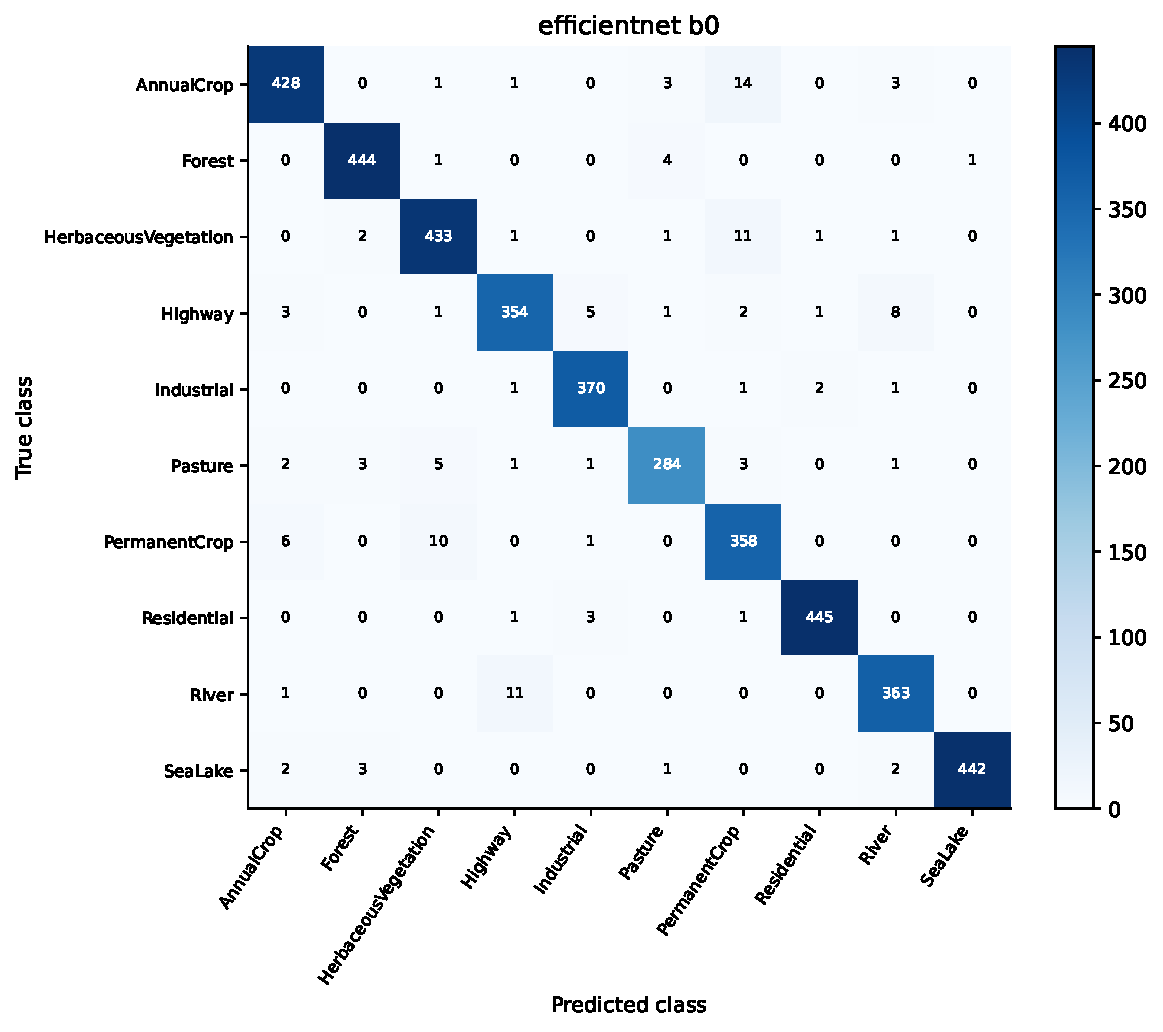
\includegraphics[width=.72\textwidth]{figures/efficientnet_b0.pdf}
\caption{EfficientNet-B0 test confusion matrix (counts).}
\label{fig:efficientnet_b0_cm}
\end{figure}

\section{Final Comparison}
\label{sec:comparison}
\subsection{Accuracy}
Figure~\ref{fig:final_accuracy} compares all four validation-selected
checkpoints. Both pretrained models outperform the custom networks on this
test set. For Model B, the question is whether that improvement justifies
the additional storage and computation for the intended device.
\begin{figure}[H]\centering
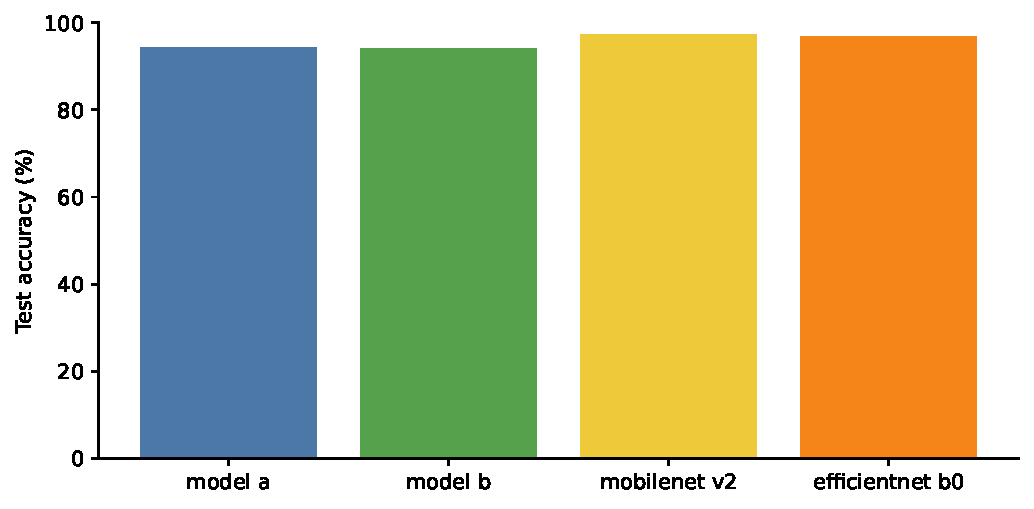
\includegraphics[width=0.96\textwidth]{figures/final_accuracy.pdf}
\caption{Held-out test accuracy using validation-selected checkpoints.}
\label{fig:final_accuracy}
\end{figure}
Relative to MobileNetV2, Model B gives \MobileAccuracyGap{} percentage points
lower test accuracy; relative to EfficientNet-B0, the difference is
\EfficientAccuracyGap{} percentage points. These are observed accuracy costs
under the tested configurations.
\subsection{Parameter Count}
The parameter totals count learned tensors only, while trainable totals reflect
the active training stage. Frozen pretraining parameters still occupy storage.
Tables~\ref{tab:custom_resources} and~\ref{tab:pretrained_resources} show
\BParams{} parameters for Model B, compared with \MobileParams{} for
MobileNetV2 and \EfficientParams{} for EfficientNet-B0. Model B saves
\MobileParamSaving\% and \EfficientParamSaving\%, respectively. Freezing
feature weights reduces the trainable count but does not remove their storage
or inference cost.
\subsection{Memory Footprint}
Figure~\ref{fig:final_resources} separates parameter count from serialized
size. Model B occupies \BSizeMiB{} MiB, compared with \MobileSizeMiB{} MiB
for MobileNetV2 and \EfficientSizeMiB{} MiB for EfficientNet-B0. These are
reductions of \MobileStorageSaving\% and \EfficientStorageSaving\%.
Serialization and buffers explain why byte reductions differ from parameter
reductions.
\begin{figure}[H]\centering
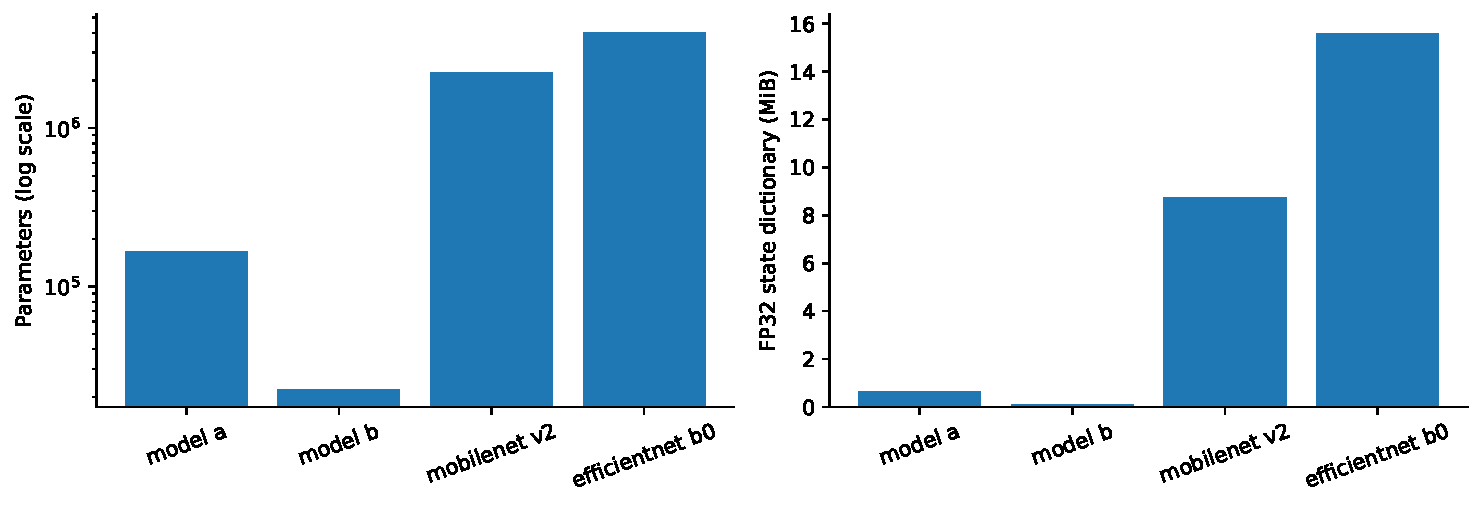
\includegraphics[width=0.96\textwidth]{figures/final_resources.pdf}
\caption{Parameter counts and measured FP32 state-dictionary sizes.}
\label{fig:final_resources}
\end{figure}

Sizes include batch-normalization buffers and serialization overhead but exclude
optimizer state. KiB and MiB use powers of 1024. The CSV column suffixes
\texttt{kb/mb} use these binary units. Disk size is not peak inference RAM;
activation and workspace memory are not measured.
\subsection{Computational Cost}
Table~\ref{tab:compute} compares one-image arithmetic counts with measured
CPU latency. Model B uses \MobileMacSaving\% fewer counted MACs than
MobileNetV2 and \EfficientMacSaving\% fewer than EfficientNet-B0. These
savings concern Conv2d and Linear operations only.
% Generated from saved experiment evidence; do not edit values.
\begin{table}[H]\centering\small
\caption{One 64x64 image: Conv/Linear arithmetic estimates and batch-one host CPU latency.}\label{tab:compute}
\begin{tabular}{lrrrr}
\toprule
Model & MACs (M) & 2xMAC (MFLOP) & CPU mean (ms) & CPU p95 (ms) \\ \midrule
Model A & 30.967 & 61.934 & 1.358 & 1.802 \\
Model B & 6.188 & 12.377 & 1.723 & 2.459 \\
MobileNetV2 & 24.461 & 48.923 & 8.452 & 13.143 \\
EfficientNet-B0 & 31.979 & 63.959 & 12.454 & 27.092 \\
\bottomrule
\end{tabular}
\end{table}


MAC accounting uses forward hooks to obtain executed layer output shapes,
kernel sizes and group counts, avoiding an external profiling dependency.
It excludes normalization, activations, pooling, residual additions and data
movement; twice MACs is only an arithmetic FLOP estimate. CPU timing uses the
Intel Core i7-13620H host, four PyTorch threads, FP32, batch one, 20 warm-ups
and 100 timed forwards. It excludes preprocessing and file I/O.
The preallocated benchmark input is a zero tensor of the required shape;
this is a forward-pass microbenchmark, not end-to-end application latency.
GPU epoch times and CPU inference times measure different workloads.
In Table~\ref{tab:compute}, Model B takes \BLatency{} ms on average versus
\ALatency{} ms for Model A despite its lower MAC count. MobileNetV2 and
EfficientNet-B0 take \MobileLatency{} ms and \EfficientLatency{} ms,
respectively.
\subsection{Edge Deployment Trade-offs}
Model B is a reasonable candidate when weight storage is the main constraint
and its accuracy cost is acceptable. Model A remains competitive when the
target resembles the measured host and latency matters more than checkpoint
size: it is faster here and has slightly higher test accuracy. MobileNetV2
is the stronger pretrained candidate in these experiments because it combines
higher accuracy with lower storage and host latency than EfficientNet-B0.
This conclusion is limited to the current split and schedule.

The pretrained models require more time per epoch, especially after unfreezing
(Table~\ref{tab:transfer_stages}). Their shorter fine-tuning schedules do not
include the original ImageNet training cost. Neither MAC counts nor host
measurements establish performance on an edge accelerator. Target-device
operator support, quantization, peak RAM, latency and power should be checked
before deployment. The present evidence establishes storage and arithmetic
savings, not energy savings.

\section{Discussion}
\label{sec:discussion}
The custom comparison holds channel widths, pooling schedule, training budget
and optimizer fixed, while Model B introduces depthwise/pointwise factorization
and additional normalization and ReLU operations. Thus the observed difference
cannot be attributed solely to the convolution operator. Both custom models
show validation fluctuations, making the saved best checkpoint preferable to
blindly using the final epoch.
The class-level errors explain why aggregate metrics should be read together.
In Figure~\ref{fig:model_a_cm}, 50 HerbaceousVegetation images are predicted as
PermanentCrop, contributing to PermanentCrop precision of
\APermanentPrecision\%. In Figure~\ref{fig:model_b_cm}, 22 Highway images are
predicted as Industrial; Highway recall is \BHighwayRecall\%. Model B thus
changes the error distribution rather than uniformly reducing performance.

In Figure~\ref{fig:mobilenet_v2_cm}, the largest directed confusion count is
10, shared by PermanentCrop predicted as HerbaceousVegetation and River
predicted as Highway. EfficientNet-B0's largest directed confusion is 14
AnnualCrop images predicted as PermanentCrop
(Figure~\ref{fig:efficientnet_b0_cm}). Crop categories may share colour and
texture at this resolution, but image-level analysis would be needed to
establish the causes. The matrices show which errors occur, not why they occur.

These are single-seed observations with no confidence intervals or repeated-run
variance estimate. Small accuracy differences should not be treated as proven
general advantages. The split is stratified but not geographic; satellite
scene correlation can make generalization to new regions harder than this
test suggests. ImageNet transfer supplies additional prior information, and
the 64x64 input differs from the pretrained recipe. These results are not the
best attainable performance of the pretrained architectures. The optimizer pilot compares
three fixed configurations for a short budget; it does not prove universal
optimizer superiority. No unseen edge device or energy benefit is asserted.

\section{Conclusion}
The custom resource-constrained model meets the parameter requirement with
\BParams{} trainable parameters and \BAccuracy\% test accuracy. Relative to
Model A, it saves \ParamReduction\% of parameters and \MacReduction\% of
counted MACs at an observed accuracy cost of \CustomAccuracyGap{} percentage
points, although host timing does not improve. Momentum improves the tested
SGD recipe, while Adam gives the strongest validation result and is used for
both final custom runs. MobileNetV2 achieves the highest observed test
accuracy, \MobileAccuracy\%, at a larger storage cost. The preferred model
therefore depends on weight-storage capacity, acceptable accuracy loss and
measured target-device performance, rather than parameter count alone.

\clearpage
\bibliographystyle{plain}
\bibliography{references}
\clearpage
\appendix
\section{Layer-wise Architecture Tables}
\label{app:architectures}
The alias \texttt{f} means \texttt{features}; \texttt{head} means
\texttt{classifier}. Shapes include batch size one. Input/output shapes expose
all channel counts. K/S/P denotes kernel/stride/padding; symmetric pairs use
\texttt{x}. A dash denotes not applicable. All listed parameters are trainable.
NCHW means batch, channels, height and width; thus each row gives input and
output channel counts. A convolution has as many filters as output channels.
ReLU rows show activation placement; convolution and linear entries have no
implicit activation. BN denotes batch normalization
and GAP denotes adaptive global average pooling. Model B depthwise convolutions
use groups equal to input channels; its pointwise and all standard convolutions
use one group. DWConv and PWConv denote depthwise and pointwise convolutions.
Full names and groups are in the machine-readable architecture CSVs.
\subsection{Model A}
Table~\ref{tab:model_a_layers} gives the complete standard CNN, including
normalization scales/offsets and the classifier bias in its parameter sum.
\begingroup\scriptsize\setlength{\tabcolsep}{3pt}
\begin{longtable}{lllllr}
\caption{Model A leaf layers, shapes and trainable parameter counts.}\label{tab:model_a_layers}\\
\toprule Layer & Operation & Input (NCHW) & Output & K/S/P & Params \\ \midrule\endfirsthead
\multicolumn{6}{l}{Model A layers (continued)}\\\toprule Layer & Operation & Input (NCHW) & Output & K/S/P & Params \\ \midrule\endhead
f.0.0 & Conv2d & $1\times3\times64\times64$ & $1\times24\times64\times64$ & 3x3/1x1/1x1 & 648 \\
f.0.1 & BN & $1\times24\times64\times64$ & $1\times24\times64\times64$ & -/-/- & 48 \\
f.0.2 & ReLU & $1\times24\times64\times64$ & $1\times24\times64\times64$ & -/-/- & 0 \\
f.0.3 & MaxPool & $1\times24\times64\times64$ & $1\times24\times32\times32$ & 2/2/0 & 0 \\
f.1.0 & Conv2d & $1\times24\times32\times32$ & $1\times48\times32\times32$ & 3x3/1x1/1x1 & 10368 \\
f.1.1 & BN & $1\times48\times32\times32$ & $1\times48\times32\times32$ & -/-/- & 96 \\
f.1.2 & ReLU & $1\times48\times32\times32$ & $1\times48\times32\times32$ & -/-/- & 0 \\
f.1.3 & MaxPool & $1\times48\times32\times32$ & $1\times48\times16\times16$ & 2/2/0 & 0 \\
f.2.0 & Conv2d & $1\times48\times16\times16$ & $1\times96\times16\times16$ & 3x3/1x1/1x1 & 41472 \\
f.2.1 & BN & $1\times96\times16\times16$ & $1\times96\times16\times16$ & -/-/- & 192 \\
f.2.2 & ReLU & $1\times96\times16\times16$ & $1\times96\times16\times16$ & -/-/- & 0 \\
f.2.3 & MaxPool & $1\times96\times16\times16$ & $1\times96\times8\times8$ & 2/2/0 & 0 \\
f.3.0 & Conv2d & $1\times96\times8\times8$ & $1\times128\times8\times8$ & 3x3/1x1/1x1 & 110592 \\
f.3.1 & BN & $1\times128\times8\times8$ & $1\times128\times8\times8$ & -/-/- & 256 \\
f.3.2 & ReLU & $1\times128\times8\times8$ & $1\times128\times8\times8$ & -/-/- & 0 \\
f.3.3 & MaxPool & $1\times128\times8\times8$ & $1\times128\times4\times4$ & 2/2/0 & 0 \\
pool & GAP & $1\times128\times4\times4$ & $1\times128\times1\times1$ & -/-/- & 0 \\
flatten & Flatten & $1\times128\times1\times1$ & $1\times128$ & -/-/- & 0 \\
head & Linear & $1\times128$ & $1\times10$ & -/-/- & 1290 \\
\midrule\multicolumn{5}{r}{Total trainable parameters} & 164,962 \\ \bottomrule
\end{longtable}
\endgroup

\clearpage
\subsection{Model B}
Table~\ref{tab:model_b_layers} gives the complete depthwise-separable CNN.
The layer sum independently verifies the parameter budget.
\begingroup\scriptsize\setlength{\tabcolsep}{3pt}
\begin{longtable}{lllllr}
\caption{Model B leaf layers, shapes and trainable parameter counts.}\label{tab:model_b_layers}\\
\toprule Layer & Operation & Input (NCHW) & Output & K/S/P & Params \\ \midrule\endfirsthead
\multicolumn{6}{l}{Model B layers (continued)}\\\toprule Layer & Operation & Input (NCHW) & Output & K/S/P & Params \\ \midrule\endhead
f.0.0 & Conv2d & $1\times3\times64\times64$ & $1\times24\times64\times64$ & 3x3/1x1/1x1 & 648 \\
f.0.1 & BN & $1\times24\times64\times64$ & $1\times24\times64\times64$ & -/-/- & 48 \\
f.0.2 & ReLU & $1\times24\times64\times64$ & $1\times24\times64\times64$ & -/-/- & 0 \\
f.0.3 & MaxPool & $1\times24\times64\times64$ & $1\times24\times32\times32$ & 2/2/0 & 0 \\
f.1.0.0 & DWConv & $1\times24\times32\times32$ & $1\times24\times32\times32$ & 3x3/1x1/1x1 & 216 \\
f.1.0.1 & BN & $1\times24\times32\times32$ & $1\times24\times32\times32$ & -/-/- & 48 \\
f.1.0.2 & ReLU & $1\times24\times32\times32$ & $1\times24\times32\times32$ & -/-/- & 0 \\
f.1.0.3 & PWConv & $1\times24\times32\times32$ & $1\times48\times32\times32$ & 1x1/1x1/0x0 & 1152 \\
f.1.0.4 & BN & $1\times48\times32\times32$ & $1\times48\times32\times32$ & -/-/- & 96 \\
f.1.0.5 & ReLU & $1\times48\times32\times32$ & $1\times48\times32\times32$ & -/-/- & 0 \\
f.1.1 & MaxPool & $1\times48\times32\times32$ & $1\times48\times16\times16$ & 2/2/0 & 0 \\
f.2.0.0 & DWConv & $1\times48\times16\times16$ & $1\times48\times16\times16$ & 3x3/1x1/1x1 & 432 \\
f.2.0.1 & BN & $1\times48\times16\times16$ & $1\times48\times16\times16$ & -/-/- & 96 \\
f.2.0.2 & ReLU & $1\times48\times16\times16$ & $1\times48\times16\times16$ & -/-/- & 0 \\
f.2.0.3 & PWConv & $1\times48\times16\times16$ & $1\times96\times16\times16$ & 1x1/1x1/0x0 & 4608 \\
f.2.0.4 & BN & $1\times96\times16\times16$ & $1\times96\times16\times16$ & -/-/- & 192 \\
f.2.0.5 & ReLU & $1\times96\times16\times16$ & $1\times96\times16\times16$ & -/-/- & 0 \\
f.2.1 & MaxPool & $1\times96\times16\times16$ & $1\times96\times8\times8$ & 2/2/0 & 0 \\
f.3.0.0 & DWConv & $1\times96\times8\times8$ & $1\times96\times8\times8$ & 3x3/1x1/1x1 & 864 \\
f.3.0.1 & BN & $1\times96\times8\times8$ & $1\times96\times8\times8$ & -/-/- & 192 \\
f.3.0.2 & ReLU & $1\times96\times8\times8$ & $1\times96\times8\times8$ & -/-/- & 0 \\
f.3.0.3 & PWConv & $1\times96\times8\times8$ & $1\times128\times8\times8$ & 1x1/1x1/0x0 & 12288 \\
f.3.0.4 & BN & $1\times128\times8\times8$ & $1\times128\times8\times8$ & -/-/- & 256 \\
f.3.0.5 & ReLU & $1\times128\times8\times8$ & $1\times128\times8\times8$ & -/-/- & 0 \\
f.3.1 & MaxPool & $1\times128\times8\times8$ & $1\times128\times4\times4$ & 2/2/0 & 0 \\
pool & GAP & $1\times128\times4\times4$ & $1\times128\times1\times1$ & -/-/- & 0 \\
flatten & Flatten & $1\times128\times1\times1$ & $1\times128$ & -/-/- & 0 \\
head & Linear & $1\times128$ & $1\times10$ & -/-/- & 1290 \\
\midrule\multicolumn{5}{r}{Total trainable parameters} & 22,426 \\ \bottomrule
\end{longtable}
\endgroup


\section{Reproducibility and Saved Evidence}
\label{app:evidence}
Before full training, checks verified dataset counts, split disjointness,
$[128,3,64,64]$ batches, all four $[2,10]$ forward-pass outputs, Model B's
parameter limit, and a short smoke training run. Metrics and plotting were
also checked. Smoke outputs are debugging artifacts and are excluded from
every experimental comparison in this report.

Table~\ref{tab:evidence} maps the main requirements to saved evidence. Final
verification recomputes test metrics from predictions, checks confusion
matrices and sample indices, and verifies model sizes, parameter counts and
history lengths. Numerical report tables derive from these files; report
formatting changes do not modify experiment files.

\begin{table}[H]\centering\small
\caption{Assignment coverage and evidence locations relative to the project root.}
\label{tab:evidence}
\begin{tabular}{>{\raggedright\arraybackslash}p{0.30\textwidth}>{\raggedright\arraybackslash}p{0.62\textwidth}}
\toprule Requirement & Saved evidence and report coverage\\\midrule
Dataset and shared split & \path{data/splits/}; Table~\ref{tab:dataset}.\\
Custom architectures and parameter limit & \path{results/tables/model_a_architecture.csv} and \path{results/tables/model_b_architecture.csv}; Tables~\ref{tab:model_a_layers} and~\ref{tab:model_b_layers}.\\
Optimizer comparison & \path{results/tables/optimizer_comparison.csv}; Tables~\ref{tab:optimizers} and~\ref{tab:optimizer_dynamics}, Figure~\ref{fig:optimizer_comparison}.\\
Custom training duration & \path{results/raw/model_a/history.csv} and \path{results/raw/model_b/history.csv}; Figures~\ref{fig:model_a_curves} and~\ref{fig:model_b_curves}.\\
Both pretrained models and staged training & \path{results/raw/mobilenet_v2/} and \path{results/raw/efficientnet_b0/}; Table~\ref{tab:transfer_stages}.\\
Test metrics and confusion matrices & Each final run directory contains \path{test_predictions.csv}, \path{classification_report.csv}, \path{confusion_matrix.csv} and \path{metrics.json}; Tables~\ref{tab:custom_accuracy} and~\ref{tab:pretrained_accuracy}.\\
Resource comparisons & \path{results/tables/custom_models.csv}, \path{results/tables/pretrained_models.csv} and \path{results/tables/final_comparison.csv}; Section~\ref{sec:comparison}.\\
Reproducibility and verification & \path{checkpoints/}, \path{README.md}, \path{RUN_LOG.md} and \path{results/verification.json}.\\
\bottomrule\end{tabular}
\end{table}

The README gives Windows setup and execution commands. Epoch count, batch
size and optimizer settings are configurable; this report describes the
recorded runs rather than unexecuted configurations. Fixed seeds and
deterministic algorithms support reproducibility in the recorded environment,
but do not guarantee bitwise equality across different software or hardware.
The saved split must be retained when reproducing or extending the experiments.

\end{document}
